\documentclass[]{article}

\usepackage[utf8]{inputenc}
\usepackage[paperheight=0.8in,paperwidth=1.4in,margin=0in]{geometry}
\usepackage{tikz}
\usetikzlibrary{shapes,arrows,automata,calc}
\usepackage{color}

\usepackage{booktabs}  % nicer table borders 

\begin{document}

%\clearpage
%\thispagestyle{empty}

\tiny{
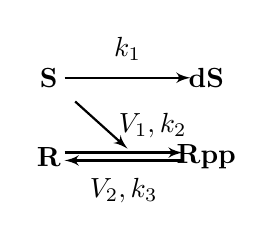
\begin{tikzpicture}[auto, outer sep=3pt, node distance=0cm,>=latex']

\node  at (-8.1, 8) (S) {$\bf S$};
\node  at (-6.1, 8) (dS) {$\bf dS$};
\draw [->, thick] ($(S)+(0.2,0)$) to node {$k_1$} ($(dS)+(-0.2,0)$);

\node  at (-8.1, 7) (R) {$\bf R$};
\node  at (-6.1, 7) (Rpp) {$\bf Rpp$};
\node  at ($(R)!0.5!(Rpp)$) (RRpp) {};
\draw [->, thick] ($(R)+(.2,.05)$) to node {} ($(Rpp)+(-0.3, .05)$);
\draw [<-, thick] ($(R)+(.2,-.05)$) to node[below] {$V_2, k_3$} ($(Rpp)+(-0.3, -.05)$);
\draw [->, thick] (S) to node[right] {$V_1, k_2$} ($(RRpp)+(0,0.1)$);
%\node  at (-3.8, 7.8) (X3) {$k_4^{cat},K_4m$};


\end{tikzpicture} 
}

\end{document}

